\section{Hadoop}

\subsection{Visitenkarte}%alles ohne Technologie
Hadoop ist ein Java basiertes Open Source Framework von Apache. 
Die Entwicklung von Hadoop wurde als Teilpojekt von Nutch angefangen. Nutch selber ist eine Weiterentwicklung von Apache Lucene. Das Ziel des Projektes Nutch war es eine schnelle Websuche, also eine Alternative zu Google, zu entwickeln. Die Herausforderung für die Nutch Entwickler war hierbei die Erstellung eines Systems, welches mit hoch skalierbaren Prozessen, Redundanzen, automatischer Fehlerbeseitigung und Lastverteilung umgehen kann. Als Google im Jahr 2004 MapReduce und das \ac{GFS} Konzept vorgestellt hat, erkannte Doug Cutting, der Erfinder von Nutch, die Vorteile und hat sie für Nutch übernommen. Im Jahr 2006 wurde Doug Cutting von Yahoo, seinem damaligen Arbeitgeber, damit beauftragt das verteilte Dateisystem und das MapReduce-Framework aus dem Nutch-Kontext zu extrahieren und in ein eigenes Framework zu überführen. So entstand Hadoop, dessen Name von dem Spielelefanten von Doug Cuttings Sohn stammt. Im Juli 2008 gewann Hadoop den Terabyte-Sort-Benchmark, was bereits damals die Reife des entstandenen Projektes zeigte. \cite[S. 24]{Wartal2012}

Mit den neuen Konzepten von Google ermöglicht Hadoop das Verteilen der Verarbeitung komplexer Prozesse über mehrere Knoten innerhalb eines Clusters.
Die Hauptziele von Hadoop sind:

\begin{itemize}
\item Erreichbarkeit: Hadoop läuft in einem großen Cluster von Rechnern oder in einer Cloud 
\item Robustheit: Wenn ein Knoten ausfällt, übernehmen andere Knoten die Verarbeitung der Daten
\item Skalierbarkeit: Hadoop skaliert linear. Es können dynamosch weitere Rechner dazugeschaltet werden, um damit die Performance des Systems zu verbessern.
\item Einfachheit: Hadoop ermöglicht eine schnelle Entwicklung der parallelen Prozesse.
\cite{HadoopInAction}
\end{itemize}

%------------------------------------------------------------------------------------------------------------------------------------------------------------------------------------------------------------------------------------------------

\subsection{Systemtechnologie}\label{hadooptech}
Hadoop besteht aus mehreren Modulen, die im Weiteren kurz beschrieben werden:

\begin{figure}[htbp] 
  \centering
     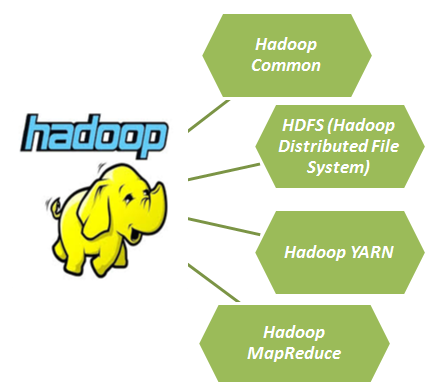
\includegraphics[width=0.5\textwidth]{images/06hadoop_modules.png}
  \caption{Hadoop-Module \cite{HaMo}}
  \label{fig: Hadoop-Module}
\end{figure}

\begin{itemize}
\item Hadoop Common: Hadoop Common stellt die Grundfunktionen bereit, die alle anderen Komponenten benötigen. Dazu zählen eine implementierungsneutrale Filesystem-Schnittstelle, die Schnittstelle für die "Remote Procedure Call"-Kommunikation im Cluster und Bibliotheken für die Serialisierung von Daten.
\item Hadoop YARN: Ein Modul für das Job-Scheduling und Cluster-Resource-Maagement
\item \ac{HDFS}: Verteiltes Dateisystem, welches einen hoch perfomanten Zugriff auf die Daten bereitstellt.
\item Hadoop MapReduce: Es ist ein auf YARN- basiertes System für die parallele Verarbeitung von riesigen Datenmenge.
\end{itemize}
Es ist möglich, Hadoop mit mehreren Dateisystemen zu betreiben: FS, HFTP FS, S3 FS etc. Das gängigste Dateisystem ist aber das \ac{HDFS}. Dieses Dateisystem basiert auf dem Google File System (\ac{GFS}). 
HDFS verwendet eine Master / Slave Architektur. Dabei verwaltet der Masterknoten (NameNode) die Metadaten von dem Dateisystem. Die Slave Knoten (DataNode) speichert die aktuellen Daten.
\subsubsection{NameNode}
Der \textit{NameNode} verwaltet alle Dateioperationen im Hadoop-Cluster. Er beinhaltet Information über die Unterteilung der Daten in Blocks und auf welcehn Knoten die Blöcke gespeichert werden.
Die Prozesse des  \textit{NameNodes} sind sehr Speicher- und I/O-lastig. Deswegen sollten \textit{NameNodes} keine Benutzerdaten speichern oder in den Berechnungsprozess eingebunden sein. Daraus resultiert, dass ein Rechner nicht gleichzeitig NameNode und DataNode sein sollte.
Zusammengefasst sind die Hauptaufgaben des NameNodes im Hadoop Dateisystem  \cite[S. XX]{Wartal2012}:
\begin{itemize}
\item Speicherung von Metadaten des Dateisystems im Hauptspeicher
\item Koordinierte Verteilung der einzelnen Datenblöcke
\item Überwachung der einzelnen Rechner-Knoten , um einen Ausfall schnell erkennen zu können
\end{itemize}

Alle Daten werden in Blöcke je 64 MB aufgeteilt. Im Vergleich zu gängigen Dateisystemen ist dies eine sehr großzügige Aufteilung. Zum Beispiel unterteilt das Linux Dateisystem alle Daten in 1KB große Blöcke. Die Aufteilung in solche großen Blöcke bei Hadoop basiert auf der Notwendigkeit sehr große Mengen an Informationen zu verarbeiten. Um einen Datenblock zu verarbeiten benötigt ein \textit{NameNode} in der Regel 150Byte Arbeitsspeicher. Demnach kann ein 1GB großer Arbeitsspeicher mehr als 6 Mio Dateien und Ordner verwalten. \cite[S. XX]{Wartal2012}
\subsubsection{DataNode}
Ein \textit{DataNode}, auch Slave-Knoten genannt, ist für die Speicherung der Daten in \ac{HDFS} verantwortlich. Er berichtet dem \textit{NameNode} über den Status der Datenverarbeitung in regelmäßigen Abständen und meldet sich bei seinem Start bei ihm an. Die Daten werden auf mehrere \textit{DataNodes} repliziert, um die Ausfallsicherheit gewährleisten zu können.
Ein\textit{DataNode} benötigt sehr viel Speicherkapazität, weil alle Daten ihm gespeichert sind \cite{nameNode}.


\subsubsection{SecondaryNameNode}
Um die Aufgabe eines \textit{SecondaryNameNodes} zu verstehen, betrachten wir kurz welche Dateien von einem \textit{NameNode} geschrieben werden und welche Probleme dabei entstehen:
\begin{figure}[H]
	\centering
	\includegraphics[width=1.0\textwidth]{images/{06.namenode}.png}
	\caption{Funktionsweise eines \textit{NameNodes}}
	\label{img:grafik-nameNode}
\end{figure}

Wie aus der Abbildung zu sehen ist, schreibt ein \textit{NameNode} zwei unterschiedliche Dateien auf die Festplatte: \\
\begin{itemize}
\item Das \textit{FsImage} ist eine Moment-Aufnahme des Dateisystem zum Zeitpunkt des Starts der \textit{NameNodes}
\item Der \textit{EditLog} beinhaltet die Änderungen, die nach dem Starten eines \textit{NameNodes} auftreten.
\end{itemize}
Ein FsImage wird nur beim Neustart eines \textit{NameNodes} erzeugt. Dabei wird die Information aus dem \textit{EditLog} in einen FsLog (FileSystem-Log) geschrieben, um die Moment-Aufnahme des Dateisystems zu speichern. Dadurch wird die Zeit für den Neustart des Systems beschleunigt.
Da in der Regel ein \textit{NameNode} nur sehr selten neu gestartet wird, entstehen folgende Probleme:
\begin{itemize}
\item Der \textit{EditLog} wird sehr groß und kann nicht verwaltet werden.
\item Das Neustarten eines \textit{NameNodes} dauert aufgrund der großen Datenmenge sehr lange.
\item Im Falle eines Ausfalls des \textit{NameNodes} geht eine sehr viele Daten verloren.
\end{itemize}

Der \textit{SecondaryNameNode} wird benötigt, um diese Probleme zu umgehen.\\
\begin{figure}[htbp]
	\centering
	\includegraphics[width=1.0\textwidth]{images/{06.secondarynamenode}.png}
	\caption{Funktionsweise eines \textit{SecondaryNameNodes}}
	\label{img:grafik-SecondaryNameNode}
\end{figure}

Die Aufgaben eines \textit{SecondaryNameNodes} sind also  \cite{secNameNode}:
\begin{itemize}
\item Daten in regelmäßigen Abständen vom \textit{EditLog} ins \textit{FsImage} verschieben.
\item Sobald ein neues \textit{FsImage}  vorhanden ist, wird es auf den \textit{NameNode} geschrieben.
\item Das neue \textit{FsImage}  wird beim nächsten Neustart des \textit{NameNodes} verwendet.
\end{itemize}

\subsubsection{Replikation der Daten in Hadoop}
Hadoop verwendet einen blockorientierten Ansatz für die Datenreplikation. Mit disem Ansatz wird jede im \ac{HDFS} abgelegte Datei in einzelne Blöcke mit einer festen Bytegröße aufgeteilt und durch den \textit{NameNode} auf unterschiedliche Cluster-Knoten abgelegt. Zusätzlich wird durch den \textit{NameNode} sichergestellt, dass jeder Block mehrfach auf unterschiedliche Knoten im Cluster repliziert wird.
In der HDFS-Standardkonfiguration repliziert der \cite{replikation} jeden Block dreifach. Kommt es nun zum Ausfall eines Knotens im Cluster, gehen nur die auf dem ausgefallenen Rechner vorhandenen Blöcke verloren und keine ganze Datei. Die verloren gegangenen Blöcke werden durch ihre Kopien auf anderen Knoten ersetzt, sodass der \textit{NameNode} die ganze Datei bereitstellen kann \cite{replikation}.


%------------------------------------------------------------------------------------------------------------------------------------------------------------------------------------------------------------------------------------------------

\subsection{Datenmodell}
In diesem Projekt wird im Bezug auf die Datenmodellierung lediglich das \ac{HDFS} aus dem Hadoop-Framework für das Speichern der Dateien genutzt. 

%------------------------------------------------------------------------------------------------------------------------------------------------------------------------------------------------------------------------------------------------

\subsection{Systeminstallation} % Installation auf der Grundlage unseres Clusters
Da Hadoop in Java implementiert ist, ist es plattformunabhängig und kann sowohl auf Windows, Linux oder MacOs installiert werden.
Im folgenden Abscnitt wird beschrieben, wie man Hadoop auf mehreren Knoten innerhalb eines Clusters installieren kann. 

Bevor man mit der Installation von Hadoop System begint, müssen zwei Voraussetzungen erfüllt werden.
\begin{enumerate}
\item Eine Java Laufzeitumgebung. Für Hadoop braucht man mindestens Java Version 1.6.
Nachdem Java auf der dafür vorgesehenen Maschine installiert ist, muss man die \textit{JAVA\_HOME}-Variable mit dem richtigen Java-Verzeichnis verknüpfen.
\item \ac{SSH} muss installiert werden und der \textit{\ac{SSH}-Daemon} muss laufen, damit die Hadoop-Scripte ausgeführt werden können.
\end{enumerate}
Als nächstes muss eine Hadoop-Distribution aus dem Internet (\url{http://hadoop.apache.org/releases.html}) geladen und für den \textit{Single}- oder \textit{MultipleMode} konfiguriert werden. Bei einer Cluster-Installation muss Hadoop auf jeden Knoten des Clusters installiert werden.
Die Konfiguration von Hadoop wird an zwei Stellen verteilt \cite{hadoopConfiguration}:
\begin{itemize}
\item Read-only default configuration - core-default.xml, hdfs-default.xml, \\yarn-default.xml and mapred-default.xml.
\item Site-specific configuration - etc/hadoop/core-site.xml,\\ etc/hadoop/hdfs-site.xml, etc/hadoop/yarn-site.xml and etc/hadoop/mapred-site.xml.
\end{itemize}


Sämtliche Konfigurationsdateien befinden sich in der Hadoop Version 2.7.3 im folgenden Verzeichnis: \textit{etc/hadoop/}:
\begin{itemize}
\item In der Datei \textit{hadoop-env} findet man einen Hinweis auf die installierte Java-Version, spezifischen Speichereinstellugen usw. 
\item Die Datei \textit{core-site.xml} beinhaltet das Verzeichnis und die Adresse des Hadoop-Dateisystems. Bei einer neuen Hadoop-Installation ist diese Datei leer und muss mit Inhalt befüllt werden.
\item Der Parameter \textit{hadoop.tmp.dir} legt fest, in welchem Verzeichnis Hadoop die benötigten Dateien für das HDFS anlegen darf.
\item Der Parameter \textit{fs.defaultFS} beschreibt den \ac{URI} des \textit{NameNodes}.
\item Die Datei \textit{hdfs-site.xml} bestimmt unter Anderem den Grad der Replikation innerhalb des \ac{HDFS}. Darüber hinaus kann man in dieser Datei den Pfad zum Verzeichnis finden, in dem die Daten vom \textit{NameNode} (\textit{dfs.namenode.name.dir}) und die Daten vom \textit{DataNode}(\textit{dfs.datanode.data.dir}) liegen.
\end{itemize}

Die vollständige Liste aller Konfigurationsparameter inklusive ihrer Default-Werte finden sich unter:

\begin{itemize}
	\item \url{https://hadoop.apache.org/docs/r2.7.2/hadoop-project-dist/
	hadoop-common/core-default.xml}
	\item \url{http://hadoop.apache.org/docs/r2.7.2/hadoop-project-dist/
	hadoop-hdfs/hdfs-default.xml}
	\item \url{https://hadoop.apache.org/docs/r2.7.2/hadoop-yarn/
	hadoop-yarn-common/yarn-default.xml}
\end{itemize}

%------------------------------------------------------------------------------------------------------------------------------------------------------------------------------------------------------------------------------------------------

\subsection{Datenschema}
Das logische Datenschema wird in Abschnitt \ref{hbase_datenschema}  beschrieben.

%------------------------------------------------------------------------------------------------------------------------------------------------------------------------------------------------------------------------------------------------

\subsection{Ad-Hoc-Zugriffsmöglichkeiten}
CRUD-Operationen können in Hadoop auch ohne HBase über einen Hive-Client durchgeführt werden. Dies war jedoch nicht Bestandteil dieses Projekts. CRUD-Operationen mit HBase werden in Abschnitt \ref{hbase_adhoc} beschrieben.
